
\documentclass{IOS-Book-Article}
\usepackage{graphicx}

\usepackage{float} % keeps tables in the exact position they occupy in the code
\usepackage{mathptmx}
\usepackage{soul}\setuldepth{article}
%\usepackage{times}
%\normalfont
%\usepackage[T1]{fontenc}
%\usepackage[mtplusscr,mtbold]{mathtime}
%
\def\hb{\hbox to 11.5 cm{}}

\begin{document}

\pagestyle{headings}
\def\thepage{}
\begin{frontmatter}              % The preamble begins here.


%\pretitle{Pretitle}
\title{Health-related content in transformer-based language models:\\ Bias in domain-specific training sets.}

\markboth{}{January 2023\hb}
%\subtitle{Subtitle}


\author[A]{\fnms{Caterina} \snm{Bonan}\orcid{0000-0002-4808-6865}%
}
and
\author[B]{\fnms{Giuseppe} \snm{Samo}\orcid{0000-0003-3449-8006}
\thanks{Corresponding Author: Giuseppe Samo, Department of Linguistics, University of Geneva, E-mail: giuseppe.samo@unige.ch; mail: Rue de Candolle 2, 1205 Geneva, Switzerland. }}
\runningauthor{Bonan \& Samo}
\address[A]{University of Cambridge}
\address[B]{University of Geneva}

\begin{abstract}
In this short communication, we implement and improve results from \cite{r1}, in which we claimed that the syntactic bias observed in general-purpose training sets urged the creation of domain-specific health-communication corpora, and predicted better performance for the latter. 
\end{abstract}

\begin{keyword}
Natural Language Processing\sep Health-content\sep 
Language Models\sep Knowledge Reproduction\sep Corpora\sep COVID-19
\end{keyword}
\end{frontmatter}
\markboth{January 2023\hb}{January 2023\hb}
%\thispagestyle{empty}
%\pagestyle{empty}

\section{Introduction}

%aggiungere articolo della Ettinger
Recent developments in Natural Language Processing have
demonstrated the ability of artificial neural language models in parsing and producing complex linguistic structures across languages. Neural language models can be queried with naturally occurring sentences compared with minimally differing ex-novo examples, allowing us to elegantly detect and quantify asymmetries between pairs of isolated conditions.
In this contribution, we explore two languages and different training set to detect forms of bias in real-world representations with respect to medical semantic-encyclopedic knowledge adopting and improving the dataset discussed in [1], which tested and detected syntactic bias of transformer-based neural language models with respect to a list of mythbusters from the World Health Organization. %rimettere la footnote?
In [1]'s conclusions, the authors aimed in future studies to detect whether the observed results was due to the type of investigated training data. Specifically, whether neural language models trained domain-specific datasets might perform better than those trained with domain-general data.


\section{Materials \& Methods}

The queried dataset is in [1] and freely accessible from a Samo et al.'repository \footnote{add link github}. 

\begin{table}[]
    \centering
    \begin{tabular}{c|c|c}
         \textsc{Language} & \textsc{Language Model} & \textsc{Training set type}\\
         English & \href{https://huggingface.co/docs/transformers/model_doc/bert}{\underline{BERT}} & Domain general (web, wiki)\\
         English & \href{https://huggingface.co/docs/transformers/model_doc/big_bird}{\underline{BigBird}} & Domain general (web, wiki)\\
         English & \href{https://huggingface.co/austinmw/distilbert-base-uncased-finetuned-health_facts}{\underline{HealthF}} & Domain specific (fact checking)\\
         English & \href{https://huggingface.co/publichealthsurveillance/PHS-BERT}{\underline{PHS}} & Domain specific (health surveillance on social media)\\
         Chinese & \href{https://huggingface.co/bert-base-chinese}{\underline{Bert}} & Domain general (web, wiki)\\
         Chinese & HealthZH & Domain specific\\
         
    \end{tabular}
    \caption{Language Models used in this paper.}
    \label{tab:my_label}
\end{table}

As developped in [1], we implemeented devised ex-novo sentences. 

The methodology is to be referred to [1].

\section{Results}

\begin{figure}[H]
    \centering
    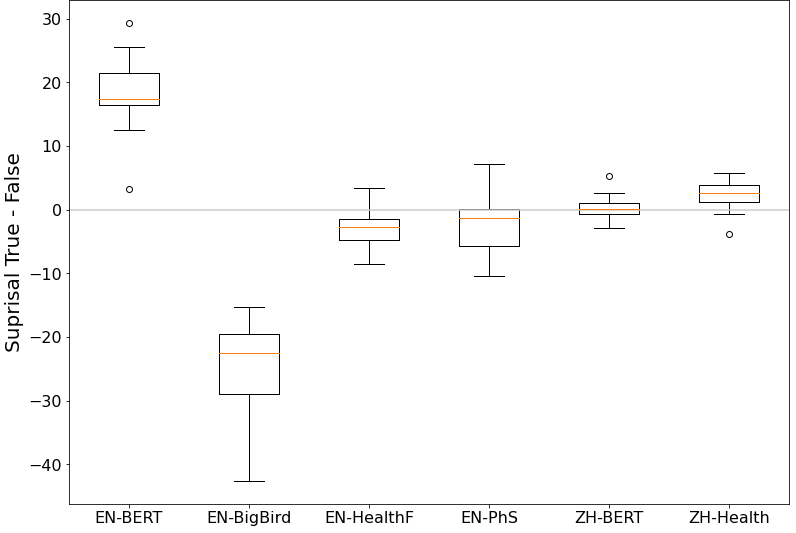
\includegraphics[scale=0.35]{graphmatplot}
    \caption{True-False across language models. The higher the results the less performing (more surprisal for true sentences) the architectures.}
    \label{fig:my_label}
\end{figure}

Our results are contrastive across langauges. We observe that the general-domain architecture (BERT) perform worse (M = 18.269, SD = 5.82 ) than domain-specific (\textit{F} (3, 64) = 177.30362; p $<$ .00001). On the other hand, the general domain performs ( \textit{M} = 0.510, \textit{SD} = 2.421) better than the domain-specific one ( \textit{M} = 1.81, \textit{SD} = 2.418) (\textit{t}(34) = 2.6837, p. < .05).

\section{Conclusions}
In this paper, we have discussed that 

\begin{thebibliography}{99}


\bibitem{r1}
Samo G, Bonan C, Si F. Health-Related Content in Transformer-Based Deep Neural Network Language Models: Exploring Cross-Linguistic Syntactic Bias. Stud Health Technol Inform. 2022 Jun 29;295:221-225. doi: 10.3233/SHTI220702. PMID: 35773848.

\bibitem{r2}
Rice AS, Farquhar-Smith WP, Bridges D, Brooks JW. Canabinoids and pain. In: Dostorovsky JO,
Carr DB, Koltzenburg M, editors. Proceedings of the 10th World Congress on Pain;  2002 Aug
17-22; San Diego, CA. Seattle (WA): IASP Press; c2003. p. 437-68, doi: ....

\end{thebibliography}
\end{document}
